\begin{frame}
	\myheading{Module 9.4 : Better initialization strategies}
\end{frame}

%%%%%%%%%%%%%%%%%%%%%%%%%%%%%%%%%%%%%%%%%%%%%%%%%%%%%%%%%%%%%%%%%%%%%%%%%%%%%%%%%%%%%%%%%
\begin{frame}
	\begin{block}{Deep Learning has evolved}
		\begin{itemize}
			\justifying
			\item \textcolor{gray}{Better optimization algorithms}
			\item \textcolor{gray}{Better regularization methods}
			\item \textcolor{gray}{Better activation functions}
			\item \textcolor{red}{Better weight initialization strategies}
		\end{itemize}
		
	\end{block}
\end{frame}

%%%%%%%%%%%%%%%%%%%%%%%%%%%%%%%%%%%%%%%%%%%%%%%%%%%%%%%%%%%%%%%%%%%%%%%%%%%%%%%%%%%%%%%%%

\begin{frame}
	
	\begin{columns}
		
		\column{0.5\textwidth}
		\begin{overlayarea}{\textwidth}{\textheight}
			
			\begin{center}
				
				\only<1->{
					\tikzstyle{input_neuron}=[circle,draw=red!50,fill=orange!10,thick,minimum size=6mm]
\tikzstyle{hidden_neuron}=[circle,draw=blue!50,fill=blue!10,thick,minimum size=1mm]
\tikzstyle{output_neuron}=[circle,draw=green!50,fill=green!20,thick,minimum size=1mm]
\tikzstyle{input}=[circle,draw=black!50,fill=black!20,thick,minimum size=1mm]

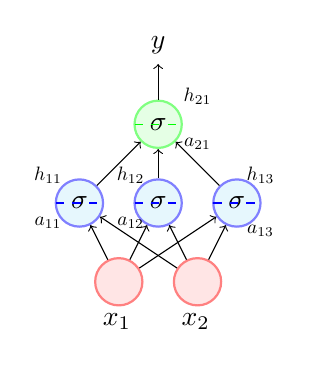
\begin{tikzpicture}
	
	\node [input_neuron] (in1) at (6.5,1)  {} ;
	\node [input_neuron] (in2) at (7.5,1)  {} ;
	%\node (input1) at (6.5,0)  {$x_{1}$};
	%\node (input2) at (7.5,0)  {$x_{2}$};
	\node (output1) at (7,4)  {$y$};
	\node [hidden_neuron] (h1) at (6,2)  {$\sigma$};
	\node [hidden_neuron] (h2) at (7,2)  {$\sigma$};
	\node [hidden_neuron] (h3) at (8,2)  {$\sigma$};
	\node [output_neuron] (o1) at (7,3)  {$\sigma$};
	
	\node[text width=0.005cm] at (6.3,0.5) {$x_{1}$};
	\node[text width=0.005cm] at (7.3,0.5) {$x_{2}$};
	
	%\draw [->] (input1) -- (in1);
	%\draw [->] (input2) -- (in2);
	
	\draw [->] (in1) -- (h1);
	\draw [->] (in1) -- (h2);
	\draw [->] (in1) -- (h3);
	\draw [->] (in2) -- (h1);
	\draw [->] (in2) -- (h2);
	\draw [->] (in2) -- (h3);
	
	\draw [->] (h1) -- (o1);
	\draw [->] (h2) -- (o1);
	\draw [->] (h3) -- (o1);
	
	\draw [->] (o1) -- (output1);
	
	\draw[green,dashed] (6.7,3) -- (7.3,3);
	\draw[blue,dashed] (5.7,2) -- (6.3,2);
	\draw[blue,dashed] (6.7,2) -- (7.3,2);
	\draw[blue,dashed] (7.7,2) -- (8.3,2);
	
	\node (formula)[scale=.7] at (7.5,3.35) {$h_{21}$};
	\node (formula)[scale=.7] at (7.5,2.75) {$a_{21}$};
	
	\node (formula)[scale=.7] at (5.6,2.35) {$h_{11}$};
	\node (formula)[scale=.7] at (6.65,2.35) {$h_{12}$};
	\node (formula)[scale=.7] at (8.3,2.35) {$h_{13}$};
	
	\node (formula)[scale=.7] at (5.6,1.75) {$a_{11}$};
	\node (formula)[scale=.7] at (6.65,1.75) {$a_{12}$};
	\node (formula)[scale=.7] at (8.3,1.65) {$a_{13}$};
	
\end{tikzpicture}
				}
				%\vspace{-0.4in}
				\begin{align*}
					\onslide<2->{a_{11}            & =w_{11}x_1+w_{12}x_{2} \\}
					\onslide<3->{a_{12}            & =w_{21}x_1+w_{22}x_{2} \\}
					\onslide<4->{\therefore a_{11} & =a_{12}=0              \\}
					\onslide<5->{\therefore h_{11} & =h_{12}}               
				\end{align*}
			\end{center}
			
		\end{overlayarea}
		
		
		\column{0.5\textwidth}
		
		\begin{overlayarea}{\textwidth}{\textheight}
			
			\only<1-5>{
				\begin{itemize}
					\justifying
					\only<1->{\item What happens if we initialize all weights to 0? }
					\only<5->{\item All neurons in layer 1 will get the same activation} 
				\end{itemize}
			}
			
			\only<6-11>{
				\begin{itemize}
					\justifying
					\only<6->{\item Now what will happen during back propagation? }
					\begin{align*}
						\onslide<7->{\nabla{w_{11}}             & =\frac{\partial \mathscr{L}(\textbf{w})}{\partial y}.\frac{\partial y}{\partial h_{11}}.\frac{\partial h_{11}}{\partial a_{11}}.x_{1} \\}
						\onslide<8->{\nabla{w_{21}}            & =\frac{\partial \mathscr{L}(\textbf{w})}{\partial y}.\frac{\partial y}{\partial h_{12}}.\frac{\partial h_{12}}{\partial a_{12}}.x_{1} \\}
						%   \onslide<11->{\nabla{w_{31}}&=\frac{\partial \mathscr{L}(\textbf{w})}{\partial y}.\frac{\partial y}{\partial h_{13}}.\frac{\partial h_{13}}{\partial a_{13}}.x_{1}\\}
						\onslide<9->{but \quad h_{11}          & =h_{12}                                                                                                                               \\}
						\onslide<10->{and\quad a_{12}           & =a_{12}                                                                                                                               \\}
						\onslide<11->{\therefore \nabla{w_{11}} & =\nabla{w_{21}}                                                                                                                       \\}
					\end{align*}
				\end{itemize}
			}
			
			\only<12->{
				\begin{itemize}
					\justifying
					\only<12->{\item Hence both the weights will get the same update and remain equal }
					\only<13->{\item Infact this symmetry will never break during training} 
					\only<14->{\item The same is true for $w_{12}$ and $w_{22}$}
					\only<15->{\item And for all weights in layer 2 (infact, work out the math and convince yourself that all the weights in this layer will remain equal )} 
					\only<16->{\item This is known as the \textbf{symmetry breaking problem} }
					\only<17->{\item This will happen if all the weights in a network are initialized to the \textbf{same value} } 
				\end{itemize}
			}
			
			
		\end{overlayarea}
		
	\end{columns}
\end{frame}

%%%%%%%%%%%%%%%%%%%%%%%%%%%%%%%%%%%%%%%%%%%%%%%%%%%%%%%%%%%%%%%%%%%%%%%%%%%%%%%%%%%%%%%%%

\begin{frame}
	\begin{columns}
		\column{0.5\textwidth}
		\begin{overlayarea}{\textwidth}{\textheight}
			\begin{figure}
				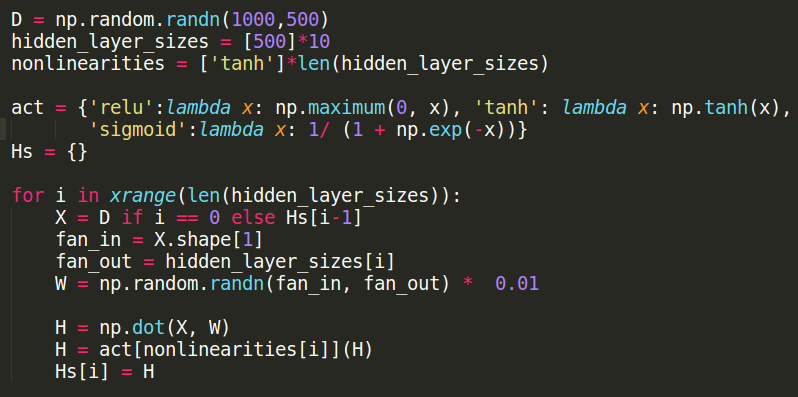
\includegraphics[width=7 cm]{images/forward.png}
			\end{figure}
			
		\end{overlayarea}
		
		\column{0.5\textwidth}
		
		\begin{overlayarea}{\textwidth}{\textheight}
			\only<1-6>{We will now consider a feedforward network with:}
			\only<2-6>{
				\begin{itemize}
					\justifying
					\only<2-6>{\item input: 1000 points, each $\in R^{500}$ }
					\only<3-6>{\item input data is drawn from unit Gaussian\\
						\newcommand\gauss[2]{1/(#2*sqrt(2*pi))*exp(-((x-#1)^2)/(2*#2^2))} % Gauss func

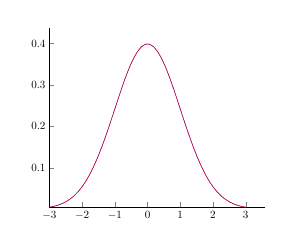
\begin{tikzpicture}[scale=.4, transform shape]

	\begin{axis}[every axis plot post/.append style={
				mark=none,domain=-3:3,samples=50}, % All plots: from -2:2, 50 samples, smooth, no marks
			axis x line*=bottom, % no box around the plot, only x and y axis
			axis y line*=left, % the * suppresses the arrow tips
		enlargelimits=upper] % extend the axes a bit to the right and top
		
		\addplot {\gauss{0}{1}};
		\addplot {\gauss{0}{1}}[scale=.5];
	\end{axis}
	
\end{tikzpicture}
					} 
					\only<4-6>{\item the network has 5 layers}
					\only<5-6>{\item each layer has 500 neurons}
					\only<6-6>{\item we will run forward propagation on this network with different weight initializations} 
				\end{itemize}
			}
		\end{overlayarea}
		
	\end{columns}
\end{frame}

%%%%%%%%%%%%%%%%%%%%%%%%%%%%%%%%%%%%%%%%%%%%%%%%%%%%%%%%%%%%%%%%%%%%%%%%%%%%%%%%%%%%%%%%%

\begin{frame}
	\begin{columns}
		\begin{column}{0.5\textwidth}
			\begin{overlayarea}{\textwidth}{\textheight}
				\only<1-3>{
					\only<1-3>{
						\begin{figure}
							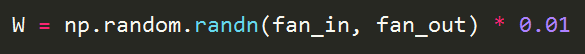
\includegraphics[scale=0.5]{images/W_01.png}
						\end{figure}}
					\only<2>{
						\begin{figure}
							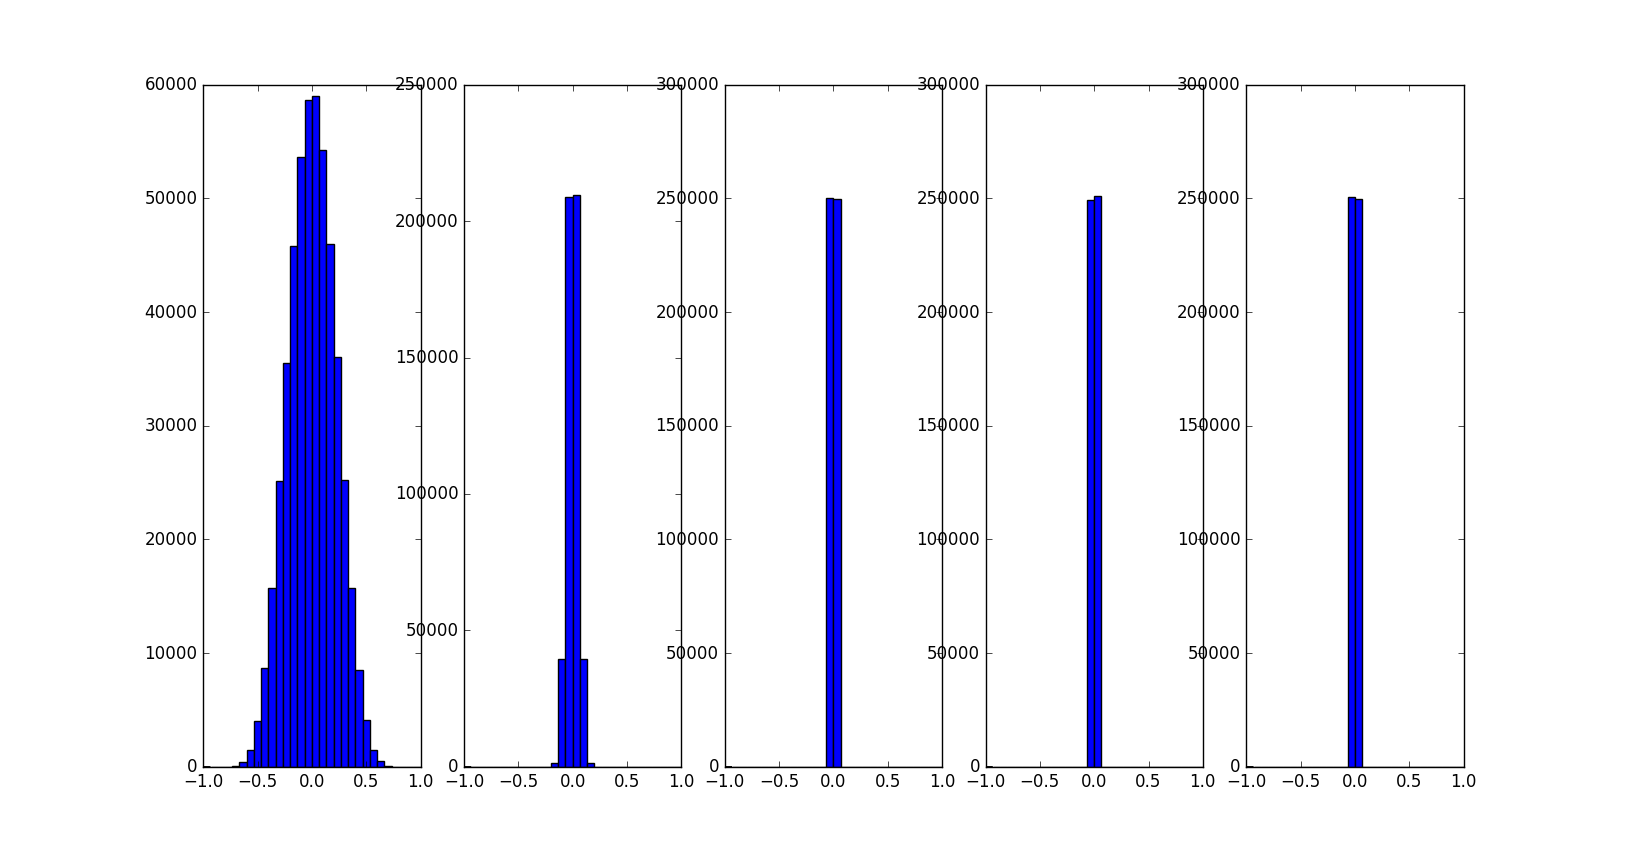
\includegraphics[scale=0.2]{images/tanh_plts_01.png}
							\caption{tanh activation functions}
						\end{figure}}
					\only<3>{
						\begin{figure}
							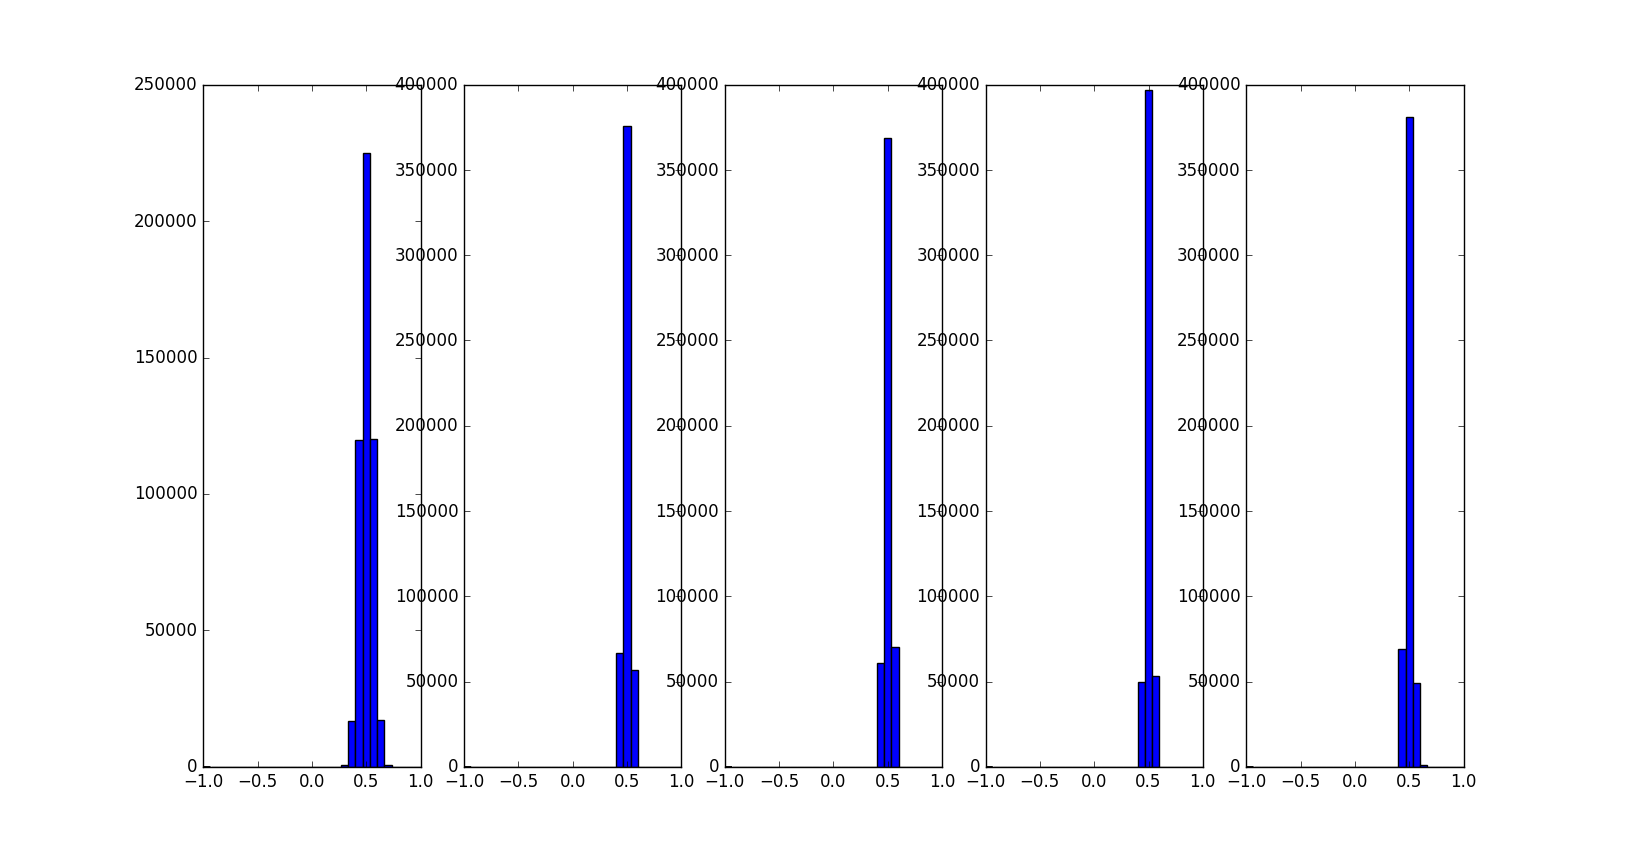
\includegraphics[scale=0.2]{images/sigm_plts_01.png}
							\caption{sigmoid activation functions}
						\end{figure}}
				}
				
			\end{overlayarea}
		\end{column}
		\begin{column}{0.5\textwidth}
			\begin{overlayarea}{\textwidth}{\textheight}
				\only<1-3>{
					\begin{itemize}
						\justifying
						\only<1->{\item Let's try to initialize the weights to small random numbers }
						\only<2-3>{\item We will see what happens to the activation across different layers } 
					\end{itemize}
				}
			\end{overlayarea}
		\end{column}
	\end{columns}
	
\end{frame}

%%%%%%%%%%%%%%%%%%%%%%%%%%%%%%%%%%%%%%%%%%%%%%%%%%%%%%%%%%%%%%%%%%%%%%%%%%%%%%%%%%%%%%%%%

\begin{frame}
	\begin{columns}
		\begin{column}{0.5\textwidth}
			\begin{overlayarea}{\textwidth}{\textheight}
				\only<4->{
					\begin{figure}
						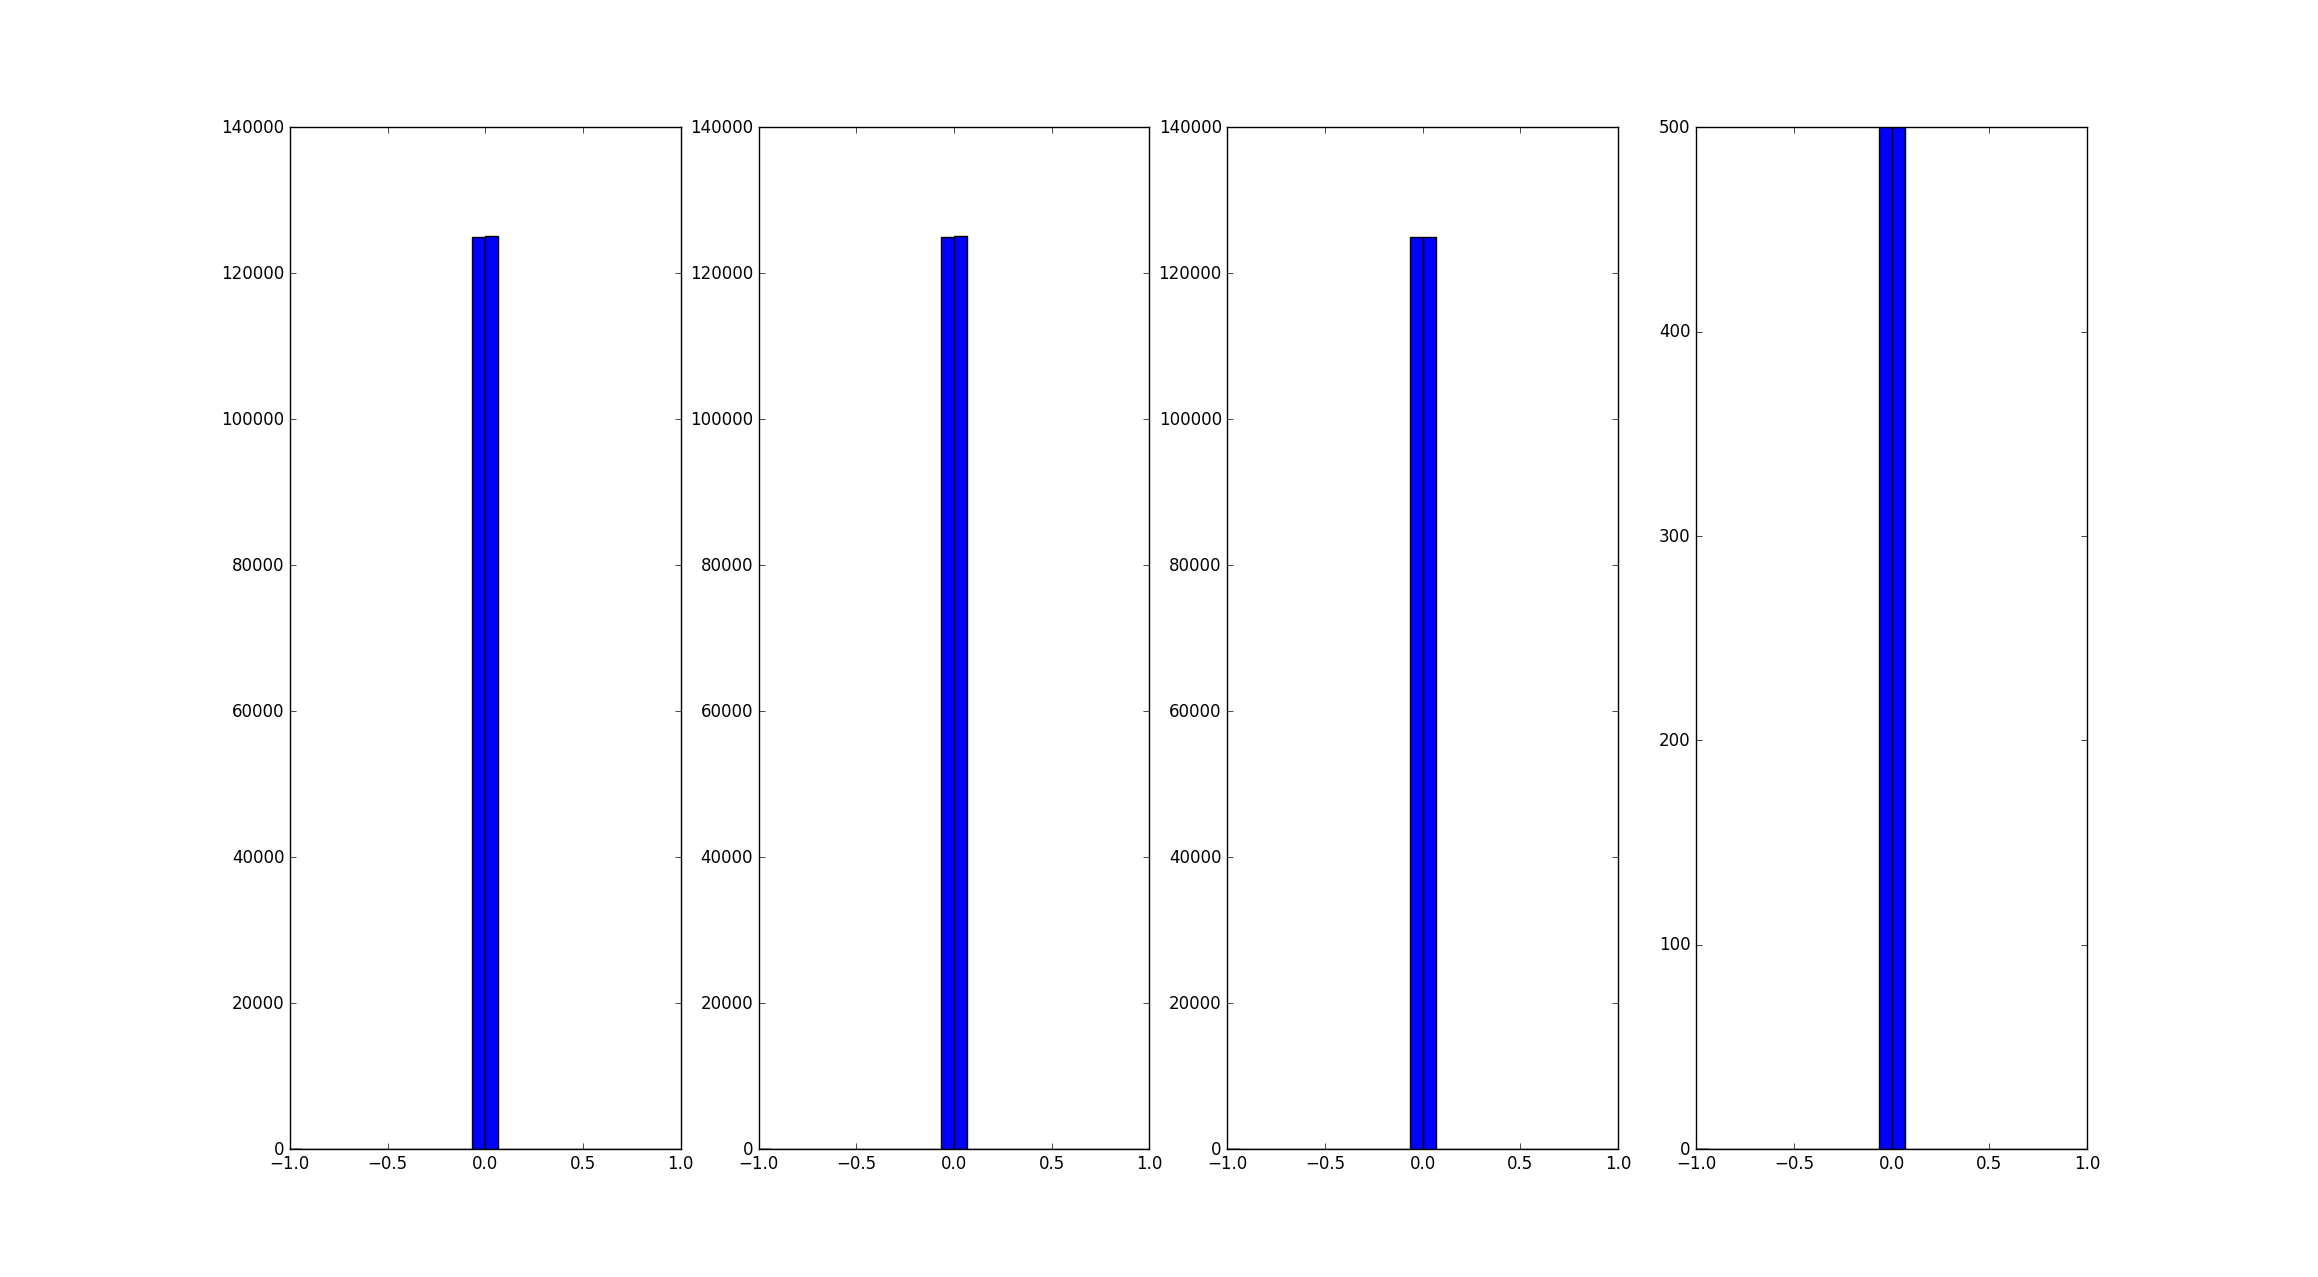
\includegraphics[scale=0.1]{images/backprop.png}
					\end{figure}}
			\end{overlayarea}
		\end{column}
		\begin{column}{0.5\textwidth}
			\begin{overlayarea}{\textwidth}{\textheight}
				
				\only<1-5>{
					\begin{itemize}
						\justifying
						\only<1->{\item What will happen during back propagation? }
						\only<2->{\item Recall that $\nabla{w_{1}}$ is proportional to the activation passing through it}
						\only<3->{\item If all the activations in a layer are very close to 0, what will happen to the gradient of the weights connecting this layer to the next layer? }
						\only<5->{\item They will all be close to 0 (vanishing gradient problem)}
					\end{itemize}
				}
			\end{overlayarea}
		\end{column}
	\end{columns}
\end{frame}

%%%%%%%%%%%%%%%%%%%%%%%%%%%%%%%%%%%%%%%%%%%%%%%%%%%%%%%%%%%%%%%%%%%%%%%%%%%%%%%%%%%%%%%%%

\begin{frame}
	\begin{columns}
		\begin{column}{0.5\textwidth}
			\begin{overlayarea}{\textwidth}{\textheight}
				\only<1-6>{
					\only<1->{
						\begin{figure}
							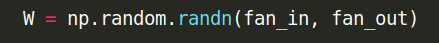
\includegraphics[scale=0.5]{images/W_1.png}
						\end{figure}
					}
					\only<3->{
						\begin{figure}
							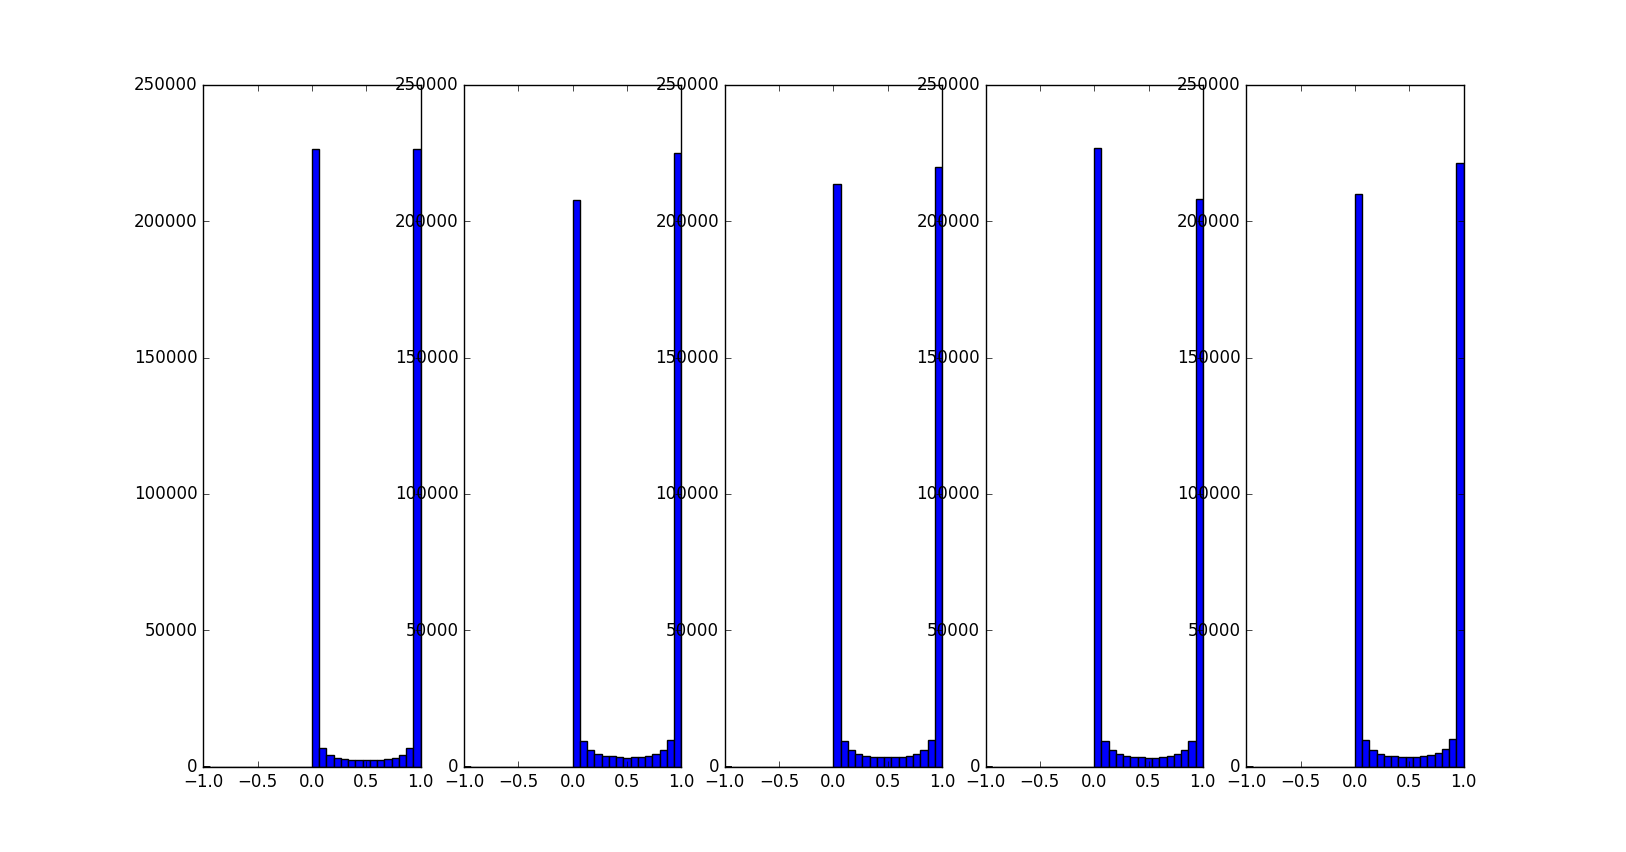
\includegraphics[scale=0.2]{images/sigm_plts_1.png}
							\caption{sigmoid activations with large weights}
						\end{figure}}
					
					\only<2->{
						\begin{figure}
							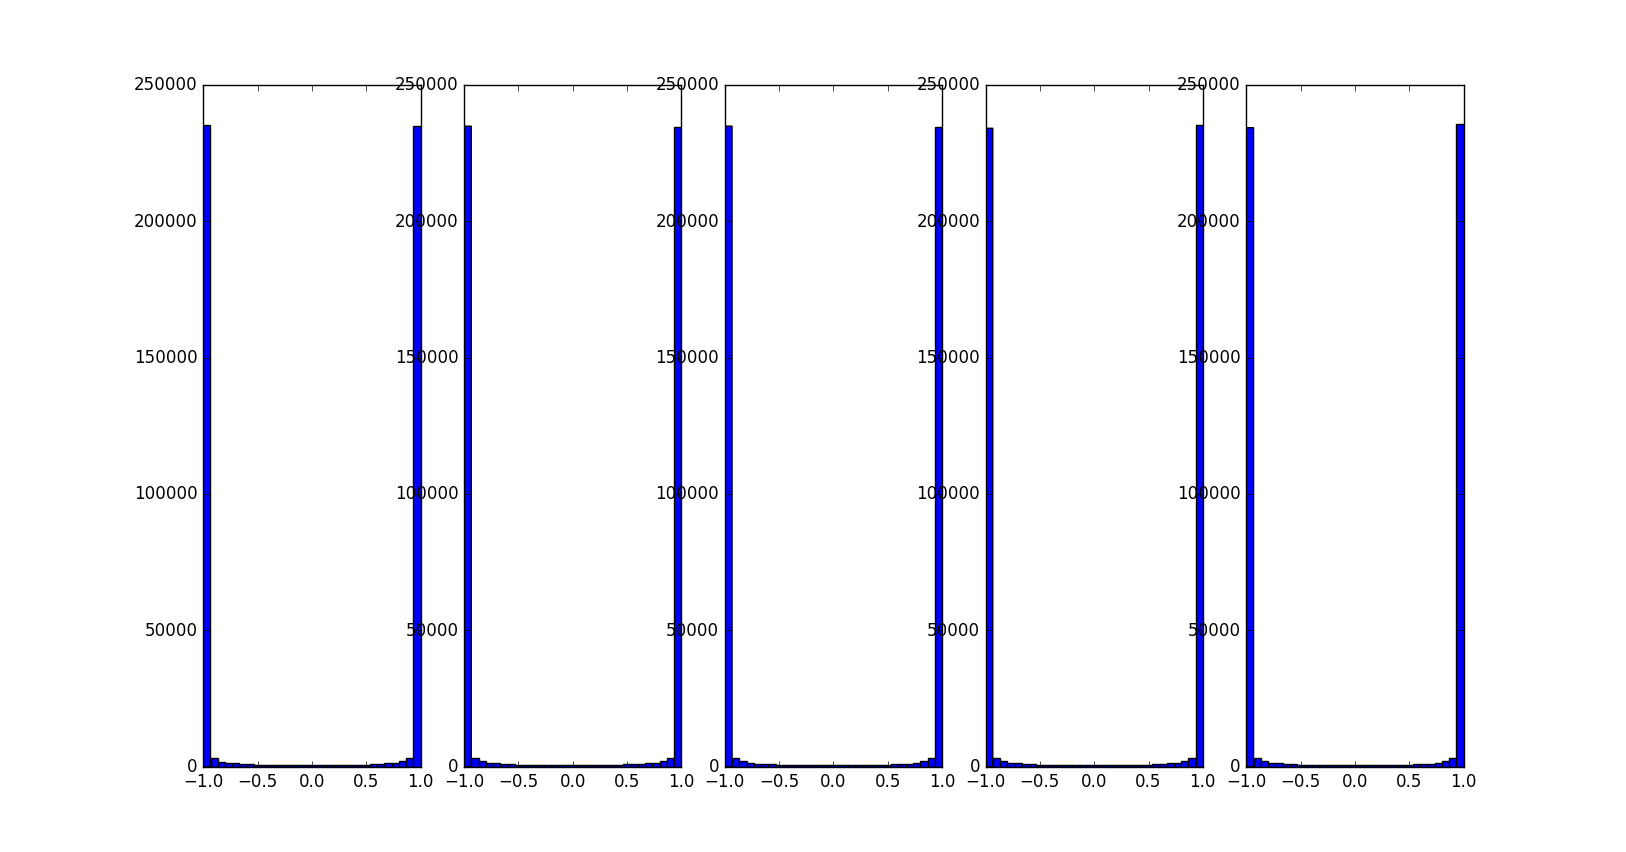
\includegraphics[scale=0.2]{images/tanh_plts_1.png}
							\caption{tanh activation with large weights}
						\end{figure}
						}
					
				}
			\end{overlayarea}
		\end{column}
		\begin{column}{0.5\textwidth}
			\begin{overlayarea}{\textwidth}{\textheight}
				
				\only<1-6>{
					\begin{itemize}
						\justifying
						\only<1->{\item Let us try to initialize the weights to large random numbers }
						\only<4->{\item Most activations have saturated}
						\only<5->{\item What happens to the gradients at saturation? }
						\only<6->{\item They will all be close to 0 (vanishing gradient problem)}
					\end{itemize}
				}
			\end{overlayarea}
		\end{column}
	\end{columns}
\end{frame}

%%%%%%%%%%%%%%%%%%%%%%%%%%%%%%%%%%%%%%%%%%%%%%%%%%%%%%%%%%%%%%%%%%%%%%%%%%%%%%%%%%%%%%%%%

\begin{frame}
	    
	\begin{columns}
		    
		\column{0.45\textwidth}
		\begin{overlayarea}{\textwidth}{\textheight}
			\vspace{1cm}
			            
			\begin{center}
				\only<2-7>{
					\tikzstyle{input_neuron}=[circle,draw=red!50,fill=red!10,thick,minimum size=6mm]
\tikzstyle{hidden_neuron}=[circle,draw=blue!50,fill=cyan!10,thick,minimum size=6mm]
\tikzstyle{output_neuron}=[circle,draw=green!50,fill=green!10,thick,minimum size=6mm]
\tikzstyle{extra_dots} = [circle,draw = black,fill=black!100,thick,minimum size=0.001mm,size=0.01cm]
\tikzstyle{input}=[circle,draw=black!50,fill=black!20,thick,minimum size=6mm]

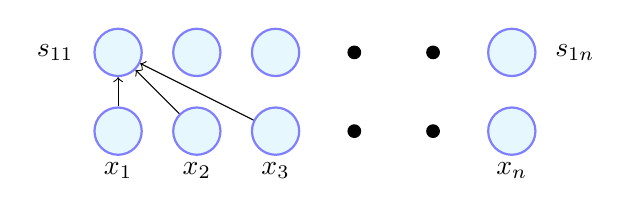
\begin{tikzpicture}	                 

	\node [hidden_neuron] (neuron11) at (3.5,7.5){}  ;
	\node(text1) at(3.5,7){$x_{1}$};
	\node [hidden_neuron] (neuron12) at (4.5,7.5) {} ;
	\node(text1) at(4.5,7){$x_{2}$};
	\node [hidden_neuron] (neuron13) at (5.5,7.5) {} ;
	\node(text1) at(5.5,7){$x_{3}$};

	\node(text) at (9.3,8.5){$s_{1n}$};
	\node(text) at (2.7,8.5){$s_{11}$};

	\node [hidden_neuron] (neuron14) at (8.5,7.5){}  ; 
	\node(text1) at(8.5,7){$x_{n}$};
	\node [hidden_neuron] (neuron21) at (3.5,8.5){}  ;
	\node [hidden_neuron] (neuron22) at (4.5,8.5)  {};
	\node [hidden_neuron] (neuron23) at (5.5,8.5)  {};
	%\node [extra_dots] (dot3) at (6.5,8.5)  ;
	\draw [black,fill=black](6.5,8.5)circle (0.8mm);
	\draw [black,fill=black](7.5,8.5)circle (0.8mm);
	\draw [black,fill=black](6.5,7.5)circle (0.8mm);
	\draw [black,fill=black](7.5,7.5)circle (0.8mm);
	%\node [extra_dots] (dot4) at (7.5,8.5)  ;
	\node [hidden_neuron] (neuron24) at (8.5,8.5){}  ; 

	\draw[->](neuron11)--(neuron21);
	\draw[->](neuron12)--(neuron21);
	\draw[->](neuron13)--(neuron21);


\end{tikzpicture}
				}
				\vspace{1cm}
				             
				\only<5->{  
					\begin{itemize}
						\justifying
						\only<5->{\item {[Assuming 0 Mean inputs and weights]}}
						\only<7->{\item {[Assuming $Var(x_{i}) = Var(x)  \forall i $ ]}}
						\only<7->{\item {[Assuming ${Var(w_{1i}) = Var(w) \forall i}$]}}
					\end{itemize}
				}			            
				            
			\end{center}
			            
			           
		\end{overlayarea}
		            
		\column{0.55\textwidth}
		\begin{overlayarea}{\textwidth}{\textheight}
			                 
			\begin{itemize}
				\justifying
				\item Let us try to arrive at a more principled way of initializing weights
			\end{itemize}
			\vspace{-0.25in}
			\begin{align*}
				\onslide<2->{s_{11}      & = \sum_{i=1}^{n} w_{1i} x_{i}}                                                \\
				\onslide<3->{Var(s_{11}) & = Var(\sum_{i=1}^{n} w_{1i}x_{i}) =  \sum_{i=1}^{n} Var(w_{1i} x_{i})}        \\
				\onslide<4->{            & =  \sum_{i=1}^{n}\big[ (E[w_{1i}])^{2} Var(x_{i}) \\
								         &+ (E[x_{i}])^{2} Var(w_{1i}) +  Var(x_{i})Var(w_{1i}) \big]}\\
				\onslide<6->{            & = \sum_{i=1}^{n} Var(x_{i}) Var(w_{1i})}\\
				\onslide<7->{            & = (n Var(w)) (Var(x))}                                                        
			\end{align*}		                   
			                 
		\end{overlayarea}
		      
		    
	\end{columns}
	    
\end{frame}

%%%%%%%%%%%%%%%%%%%%%%%%%%%%%%%%%%%%%%%%%%%%%%%%%%%%%%%%%%%%%%%%%%%%%%%%%%%%%%%%%%%%%%%%%

\begin{frame}
	\begin{columns}
		\column{0.5\textwidth}
		\begin{overlayarea}{\textwidth}{\textheight}
			\vspace{1cm}
			\begin{center}
				\tikzstyle{input_neuron}=[circle,draw=red!50,fill=red!10,thick,minimum size=6mm]
\tikzstyle{hidden_neuron}=[circle,draw=blue!50,fill=cyan!10,thick,minimum size=6mm]
\tikzstyle{output_neuron}=[circle,draw=green!50,fill=green!10,thick,minimum size=6mm]
\tikzstyle{extra_dots} = [circle,draw = black,fill=black!100,thick,minimum size=0.001mm,size=0.01cm]
\tikzstyle{input}=[circle,draw=black!50,fill=black!20,thick,minimum size=6mm]

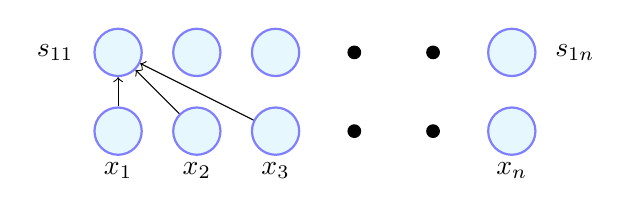
\begin{tikzpicture}	                 

	\node [hidden_neuron] (neuron11) at (3.5,7.5){}  ;
	\node(text1) at(3.5,7){$x_{1}$};
	\node [hidden_neuron] (neuron12) at (4.5,7.5) {} ;
	\node(text1) at(4.5,7){$x_{2}$};
	\node [hidden_neuron] (neuron13) at (5.5,7.5) {} ;
	\node(text1) at(5.5,7){$x_{3}$};

	\node(text) at (9.3,8.5){$s_{1n}$};
	\node(text) at (2.7,8.5){$s_{11}$};

	\node [hidden_neuron] (neuron14) at (8.5,7.5){}  ; 
	\node(text1) at(8.5,7){$x_{n}$};
	\node [hidden_neuron] (neuron21) at (3.5,8.5){}  ;
	\node [hidden_neuron] (neuron22) at (4.5,8.5)  {};
	\node [hidden_neuron] (neuron23) at (5.5,8.5)  {};
	%\node [extra_dots] (dot3) at (6.5,8.5)  ;
	\draw [black,fill=black](6.5,8.5)circle (0.8mm);
	\draw [black,fill=black](7.5,8.5)circle (0.8mm);
	\draw [black,fill=black](6.5,7.5)circle (0.8mm);
	\draw [black,fill=black](7.5,7.5)circle (0.8mm);
	%\node [extra_dots] (dot4) at (7.5,8.5)  ;
	\node [hidden_neuron] (neuron24) at (8.5,8.5){}  ; 

	\draw[->](neuron11)--(neuron21);
	\draw[->](neuron12)--(neuron21);
	\draw[->](neuron13)--(neuron21);


\end{tikzpicture}
			\end{center}
		\end{overlayarea}
		            
		            
		\column{0.5\textwidth}
		\begin{overlayarea}{\textwidth}{\textheight}
			\begin{itemize}
				\justifying
				\item In general,
				                
				      \begin{equation*}
				      	Var(S_{1i}) = (n Var(w)) (Var(x))
				      \end{equation*}
				\only<2-5>{\item What would happen if  $n Var(w) \gg 1$ ? } 
				\only<3-5>{\item The variance of $S_{1i}$ will be large}
				\only<4-5>{\item What would happen if $ n Var(w) \rightarrow 0$? }
				\only<5-5>{\item The variance of $S_{1i}$ will be small}
			\end{itemize}
                 
		\end{overlayarea}
	\end{columns}
\end{frame}
		
%%%%%%%%%%%%%%%%%%%%%%%%%%%%%%%%%%%%%%%%%%%%%%%%%%%%%%%%%%%%%%%%%%%%%%%%%%%%%%%%%%%%%%%%%
		
\begin{frame}
	\begin{columns}
		\column{0.5\textwidth}
		\begin{overlayarea}{\textwidth}{\textheight}
			\vspace{1cm}
			\only<2->{ 
				\begin{center}
					\tikzstyle{input_neuron}=[circle,draw=red!50,fill=red!10,thick,minimum size=6mm]
\tikzstyle{hidden_neuron}=[circle,draw=blue!50,fill=cyan!10,thick,minimum size=6mm]
\tikzstyle{output_neuron}=[circle,draw=green!50,fill=green!10,thick,minimum size=6mm]
\tikzstyle{extra_dots} = [circle,draw = black,fill=black!100,thick,minimum size=0.001mm,size=0.01cm]
\tikzstyle{input}=[circle,draw=black!50,fill=black!20,thick,minimum size=6mm]

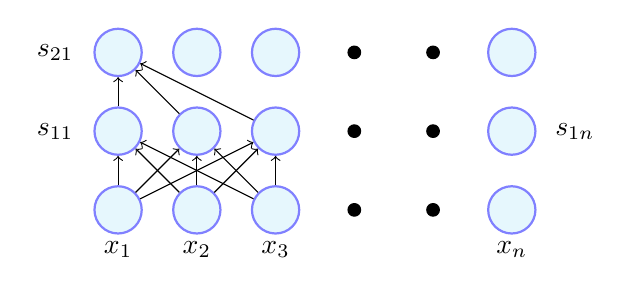
\begin{tikzpicture}

	\node [hidden_neuron] (neuron11) at (3.5,7.5) {} ;
	\node(text1) at(3.5,7){$x_1$};
	\node [hidden_neuron] (neuron12) at (4.5,7.5) {} ;
	\node(text1) at(4.5,7){$x_2$};
	\node [hidden_neuron] (neuron13) at (5.5,7.5) {} ;
	\node(text1) at(5.5,7){$x_3$};

	\node(text) at (9.3,8.5){$s_{1n}$};
	\node(text) at (2.7,8.5){$s_{11}$};
	\node(text) at (2.7,9.5){$s_{21}$};
	\node [hidden_neuron] (neuron14) at (8.5,7.5) {} ; 
	\node(text1) at(8.5,7){$x_n$};
	\node [hidden_neuron] (neuron21) at (3.5,8.5) {} ;
	\node [hidden_neuron] (neuron22) at (4.5,8.5)  {};
	\node [hidden_neuron] (neuron23) at (5.5,8.5)  {};
	\node [hidden_neuron] (neuron31) at (3.5,9.5)  {};
	\node [hidden_neuron] (neuron32) at (4.5,9.5) {} ;
	\node [hidden_neuron] (neuron33) at (5.5,9.5)  {};

	%\node [extra_dots] (dot3) at (6.5,8.5)  ;
	\draw [black,fill=black](6.5,8.5)circle (0.8mm);
	\draw [black,fill=black](7.5,8.5)circle (0.8mm);
	\draw [black,fill=black](6.5,7.5)circle (0.8mm);
	\draw [black,fill=black](7.5,7.5)circle (0.8mm);

	\draw [black,fill=black](6.5,9.5)circle (0.8mm);
	\draw [black,fill=black](7.5,9.5)circle (0.8mm);


	%\node [extra_dots] (dot4) at (7.5,8.5)  ;
	\node [hidden_neuron] (neuron24) at (8.5,8.5) {} ; 
	\node [hidden_neuron] (neuron34) at (8.5,9.5) {} ; 
	\draw[->](neuron11)--(neuron21);
	\draw[->](neuron12)--(neuron21);
	\draw[->](neuron13)--(neuron21);
	\draw[->](neuron11)--(neuron22);
	\draw[->](neuron12)--(neuron22);
	\draw[->](neuron13)--(neuron22);

	\draw[->](neuron11)--(neuron23);
	\draw[->](neuron12)--(neuron23);
	\draw[->](neuron13)--(neuron23);

	\draw[->](neuron21)--(neuron31);
	\draw[->](neuron22)--(neuron31);
	\draw[->](neuron23)--(neuron31);

\end{tikzpicture}
				\end{center}
			}
			\only<5->{ 
				\begin{equation*}
					\boxed{Var(S_{i1}) = n Var(w_1) Var(x)}
				\end{equation*}
			}
  
		\end{overlayarea}
		\column{0.5\textwidth}
		\begin{overlayarea}{\textwidth}{\textheight}
			\begin{itemize}
				\justifying
				\item<1-> Let us see what happens if we add one more layer
				\item<2-> Using the same procedure as above we will arrive at
			\end{itemize}
			\only<3->{
				\begin{equation*}
					Var(s_{21}) = \sum_{i=1}^{n} Var(s_{1i}) Var(w_{2i})
				\end{equation*}  }
			\only<4->{ \begin{equation*}
				= n Var(s_{1i}) Var(w_{2})
				\end{equation*} } 
			\only<6->{ \begin{equation*}
				Var(s_{21})\propto [n Var(w_{2})] [ n Var(w_{1})] Var(x)
				\end{equation*}}  
			\only<7->{ \begin{equation*}\propto [n Var(w)]^2 Var(x)
				\end{equation*}}  
			\only<8->{ 
				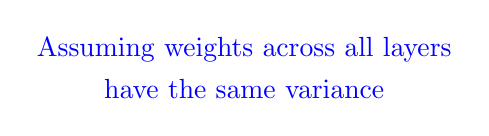
\begin{tikzpicture}
					\node[blue] (text) at (8,3.5){Assuming weights across all layers };
					\node[blue](text) at (8,3.0){have the same variance};
					%\draw[->,red,ultra thick](8,3.7) -- (8,4);
				\end{tikzpicture}
			}
  
		\end{overlayarea}
	\end{columns}

\end{frame}

%%%%%%%%%%%%%%%%%%%%%%%%%%%%%%%%%%%%%%%%%%%%%%%%%%%%%%%%%%%%%%%%%%%%%%%%%%%%%%%%%%%%%%%%%

\begin{frame}
	\begin{columns}
		\column{0.4\textwidth}
		\begin{overlayarea}{\textwidth}{\textheight}
			\vspace{2cm}
			\begin{center}
				\only<6-7>{ \begin{equation*}
					\boxed{Var(az) = a^{2}(Var(z))} 
					\end{equation*}}
			\end{center}
 
		\end{overlayarea}



		\column{0.6\textwidth}
		\begin{overlayarea}{\textwidth}{\textheight}
			\begin{itemize}
				\justifying
				\item<1-> In general,
				\only<2-7>{
					\begin{equation*}  
						Var(s_{ki}) = [n Var(w) ]^{k} Var(x)
					\end{equation*}}
				\item<3-> To ensure that variance in the output of any layer does not blow up or shrink we want:
				\only<3-7>{
					\begin{equation*}
						n\hspace{0.5mm}Var(w) = 1
					\end{equation*}
				}
				\item<4-> If we draw the weights from a unit Gaussian and scale them by $\frac{1}{\sqrt{n}}$ then, we have :
				\onslide<5-7>{\begin{align*}
					\onslide<5-7>{n Var(w) &= n\hspace{0.5mm}Var(\frac{z}{\sqrt n})}\\
					\onslide<6-7>{&= n\hspace{0.9mm}*\frac{1}{n}\hspace{0.5mm}Var(z)= 1}
					\onslide<7>{ \leftarrow (\textcolor{red}{Unit\hspace{0.4mm}Gaussian})}
					\end{align*}}
			\end{itemize}        
      
		\end{overlayarea}

	\end{columns}
\end{frame}
		
%%%%%%%%%%%%%%%%%%%%%%%%%%%%%%%%%%%%%%%%%%%%%%%%%%%%%%%%%%%%%%%%%%%%%%%%%%%%%%%%%%%%%%%%%	

\begin{frame}
	\begin{columns}
		\begin{column}{0.5\textwidth}
			\begin{overlayarea}{\textwidth}{\textheight}
				\only<1-3>{
					\only<1->{
						\begin{figure}
							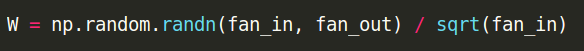
\includegraphics[scale=0.3]{./images/W_sqrt.png}
						\end{figure}
					}
					\only<3->{
						\begin{figure}
							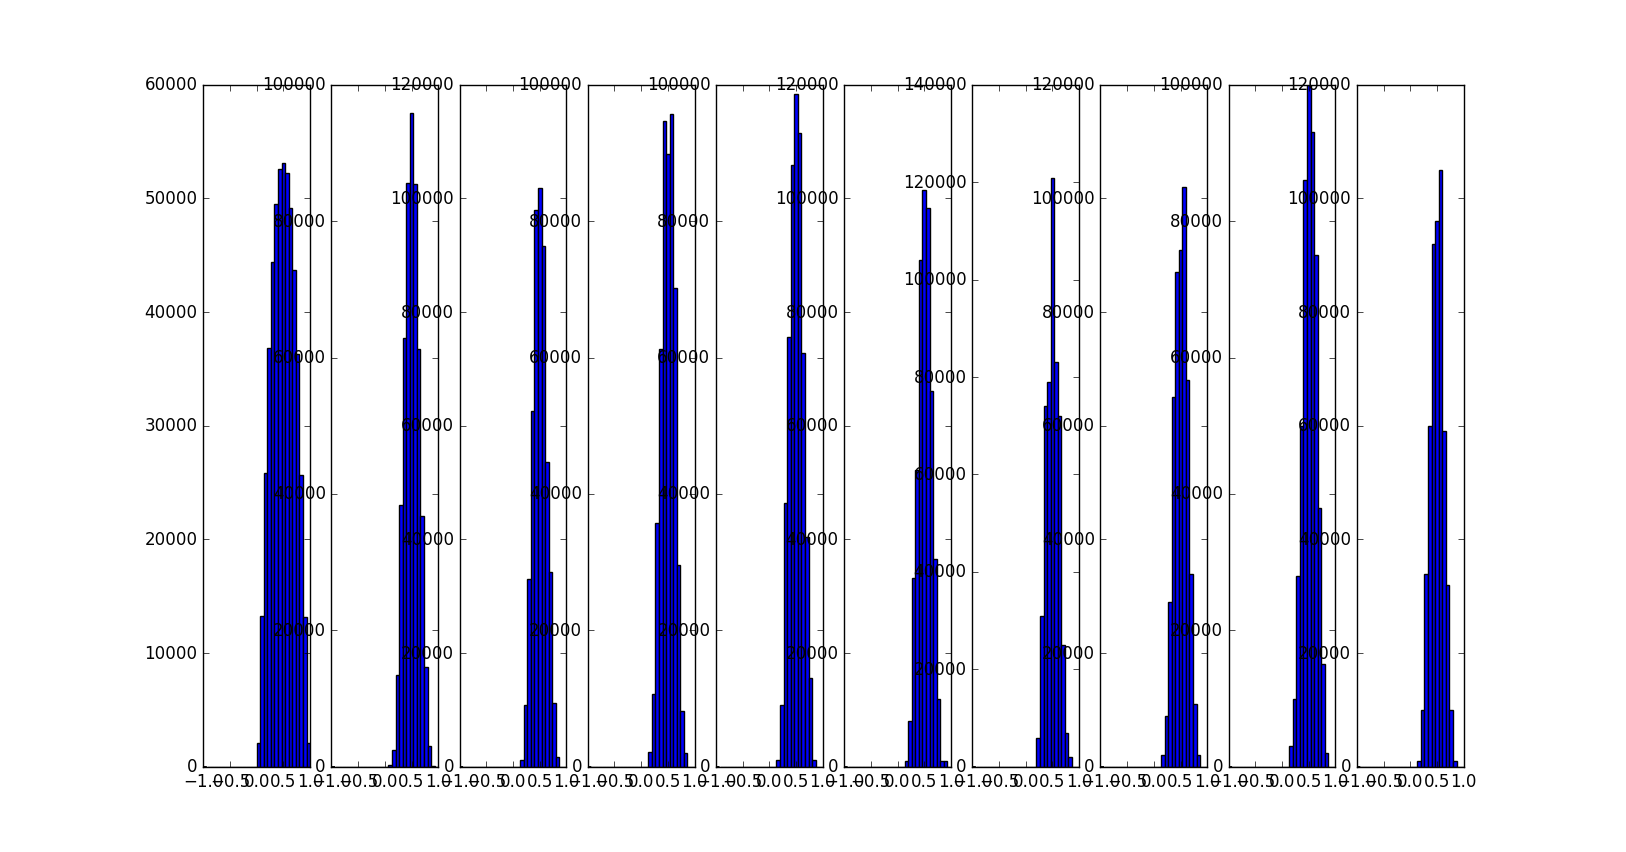
\includegraphics[scale=0.2]{./images/sigm_plts_sqrt.png}
							\caption{sigmoid activations}
						\end{figure}}
					
					\only<2->{
						\begin{figure}
							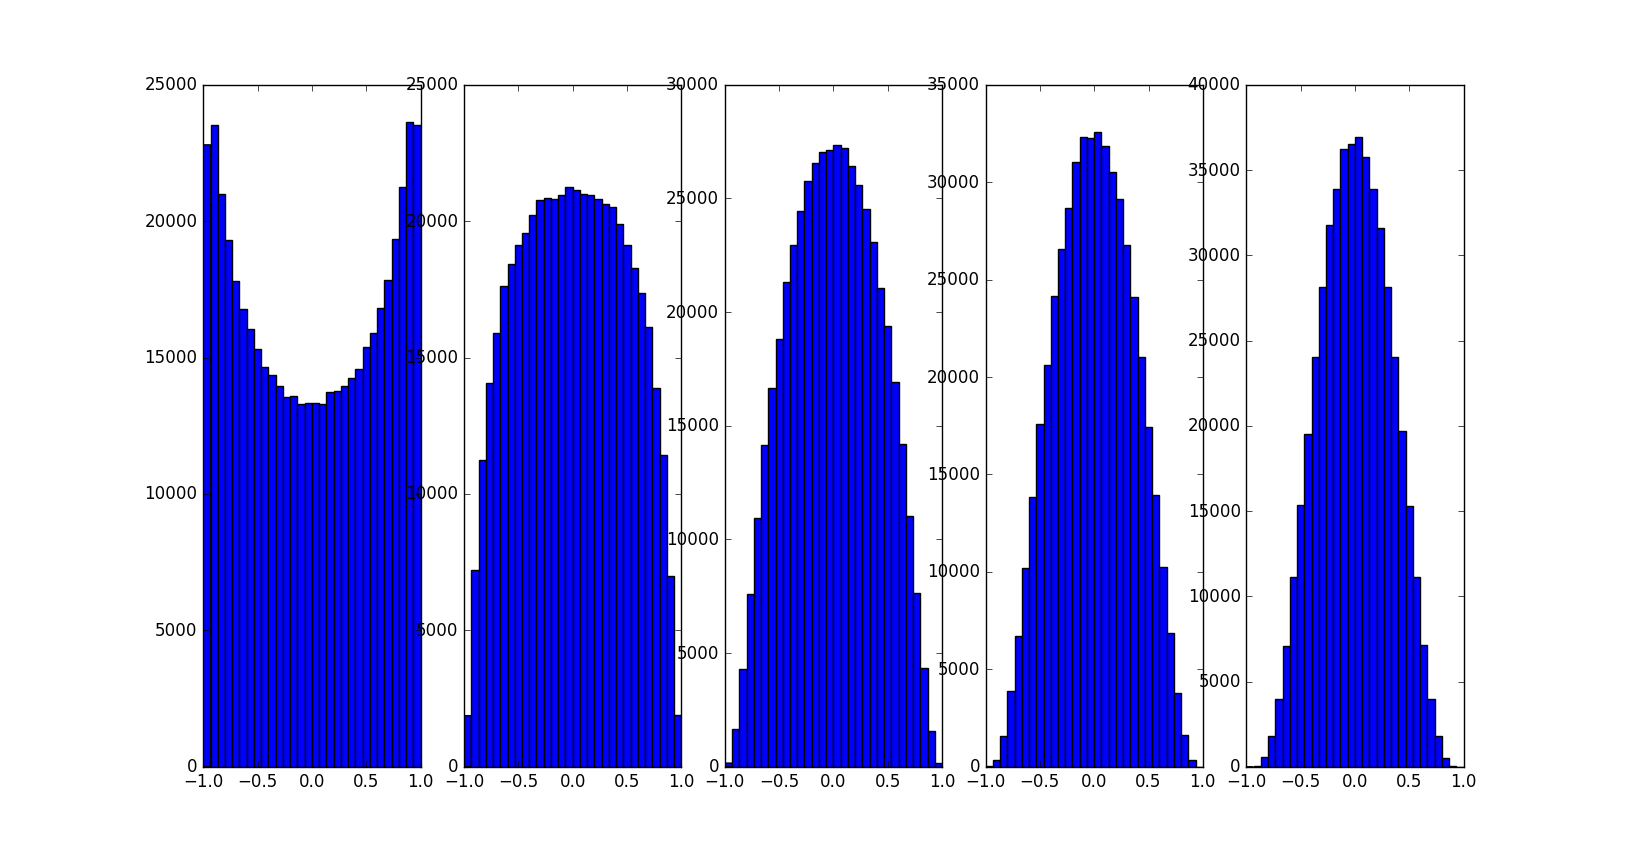
\includegraphics[scale=0.2]{./images/tanh_plts_sqrt.png}
							\caption{tanh activation}
						\end{figure}}
					
				}
			\end{overlayarea}
		\end{column}
		\begin{column}{0.5\textwidth}
			\begin{overlayarea}{\textwidth}{\textheight}
				
				\only<1-3>{
					\begin{itemize}
						\justifying
						\only<1->{\item Let's see what happens if we use this initialization}
					\end{itemize}
				}
			\end{overlayarea}
		\end{column}
	\end{columns}
\end{frame}
		
%%%%%%%%%%%%%%%%%%%%%%%%%%%%%%%%%%%%%%%%%%%%%%%%%%%%%%%%%%%%%%%%%%%%%%%%%%%%%%%%%%%%%%%%%	

\begin{frame}
	\begin{columns}
		\begin{column}{0.5\textwidth}
			\begin{overlayarea}{\textwidth}{\textheight}
				\only<1-4>{
					\only<1->{
						\begin{figure}
							%\hspace{2mm}
							\hspace*{-1.5cm}
							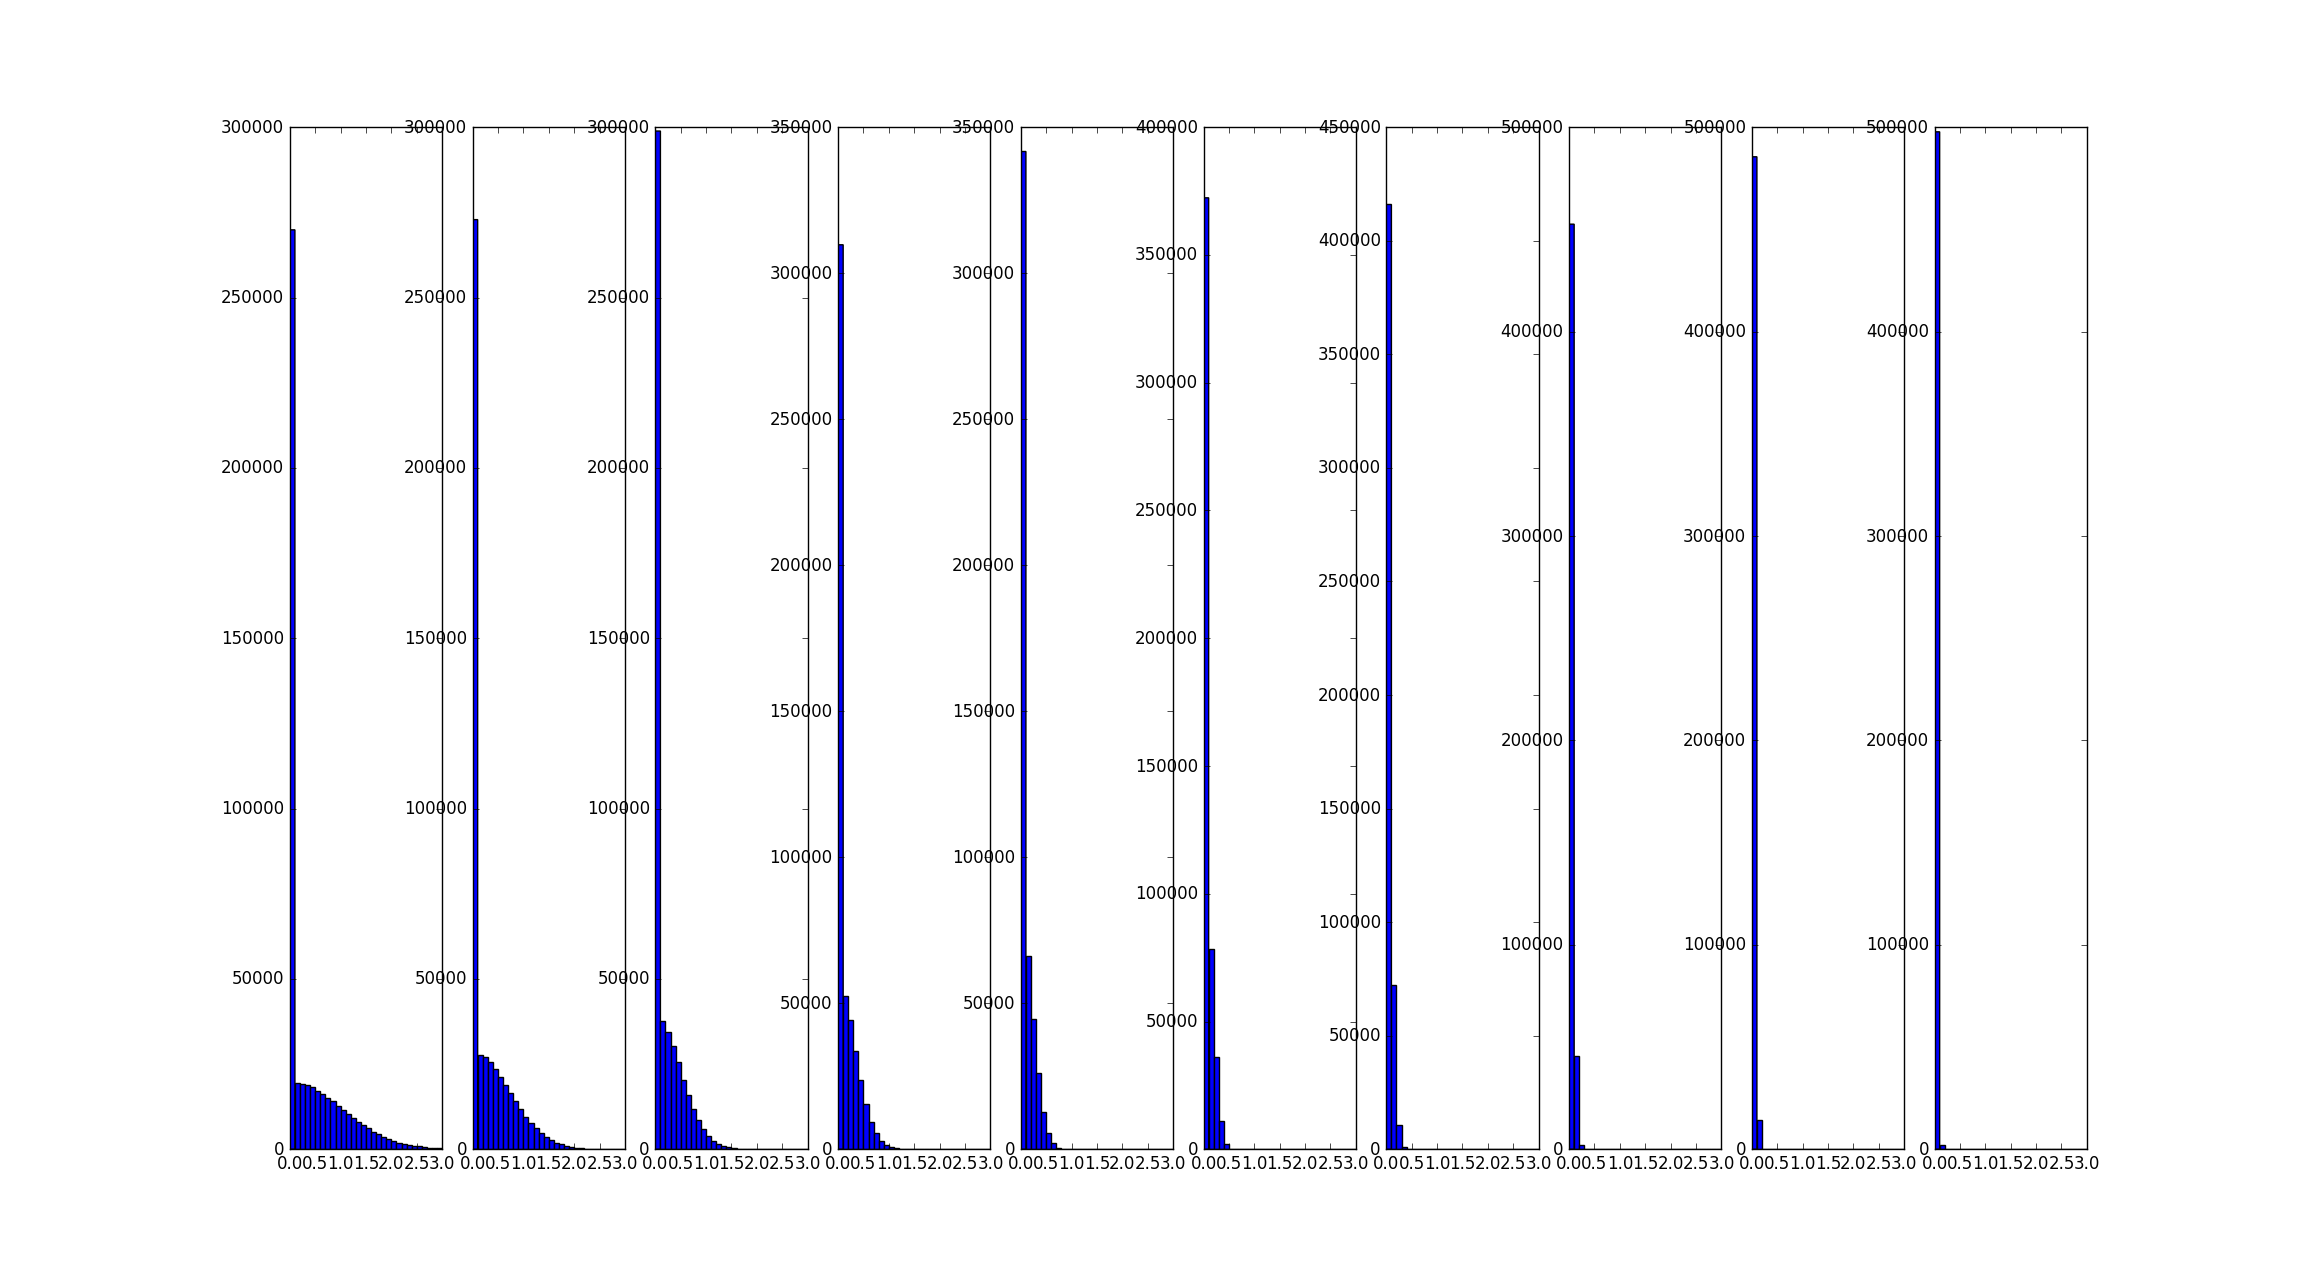
\includegraphics[scale=0.15]{./images/relu_plts_sqrt.png} 
						\end{figure}
				}}
			\end{overlayarea}
		\end{column}
		\begin{column}{0.5\textwidth}
			\begin{overlayarea}{\textwidth}{\textheight}
				
				\only<1-4>{
					\begin{itemize}
						\justifying
						\only<1->{\item However this does not work for ReLU neurons}
						\only<2->{\item Why ?}
						\only<3->{\item Intuition: \textit{He et.al.} argue that a factor of 2 is needed when dealing with ReLU Neurons}
						\only<4->{\item Intuitively this happens because the range of ReLU neurons is restricted only to the positive half of the space}
					\end{itemize}
				}
			\end{overlayarea}
		\end{column}
	\end{columns}
\end{frame}
			
%%%%%%%%%%%%%%%%%%%%%%%%%%%%%%%%%%%%%%%%%%%%%%%%%%%%%%%%%%%%%%%%%%%%%%%%%%%%%%%%%%%%%%%%%		

\begin{frame}
	\begin{columns}
		\begin{column}{0.5\textwidth}
			\begin{overlayarea}{\textwidth}{\textheight}
				\only<1-2>{
					\only<1->{
						\begin{figure}
							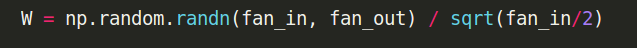
\includegraphics[scale=0.3]{./images/W_sqrt2.png}
						\end{figure}
					}
					\only<2>{
						\begin{figure}
							\hspace*{-1.5cm}
							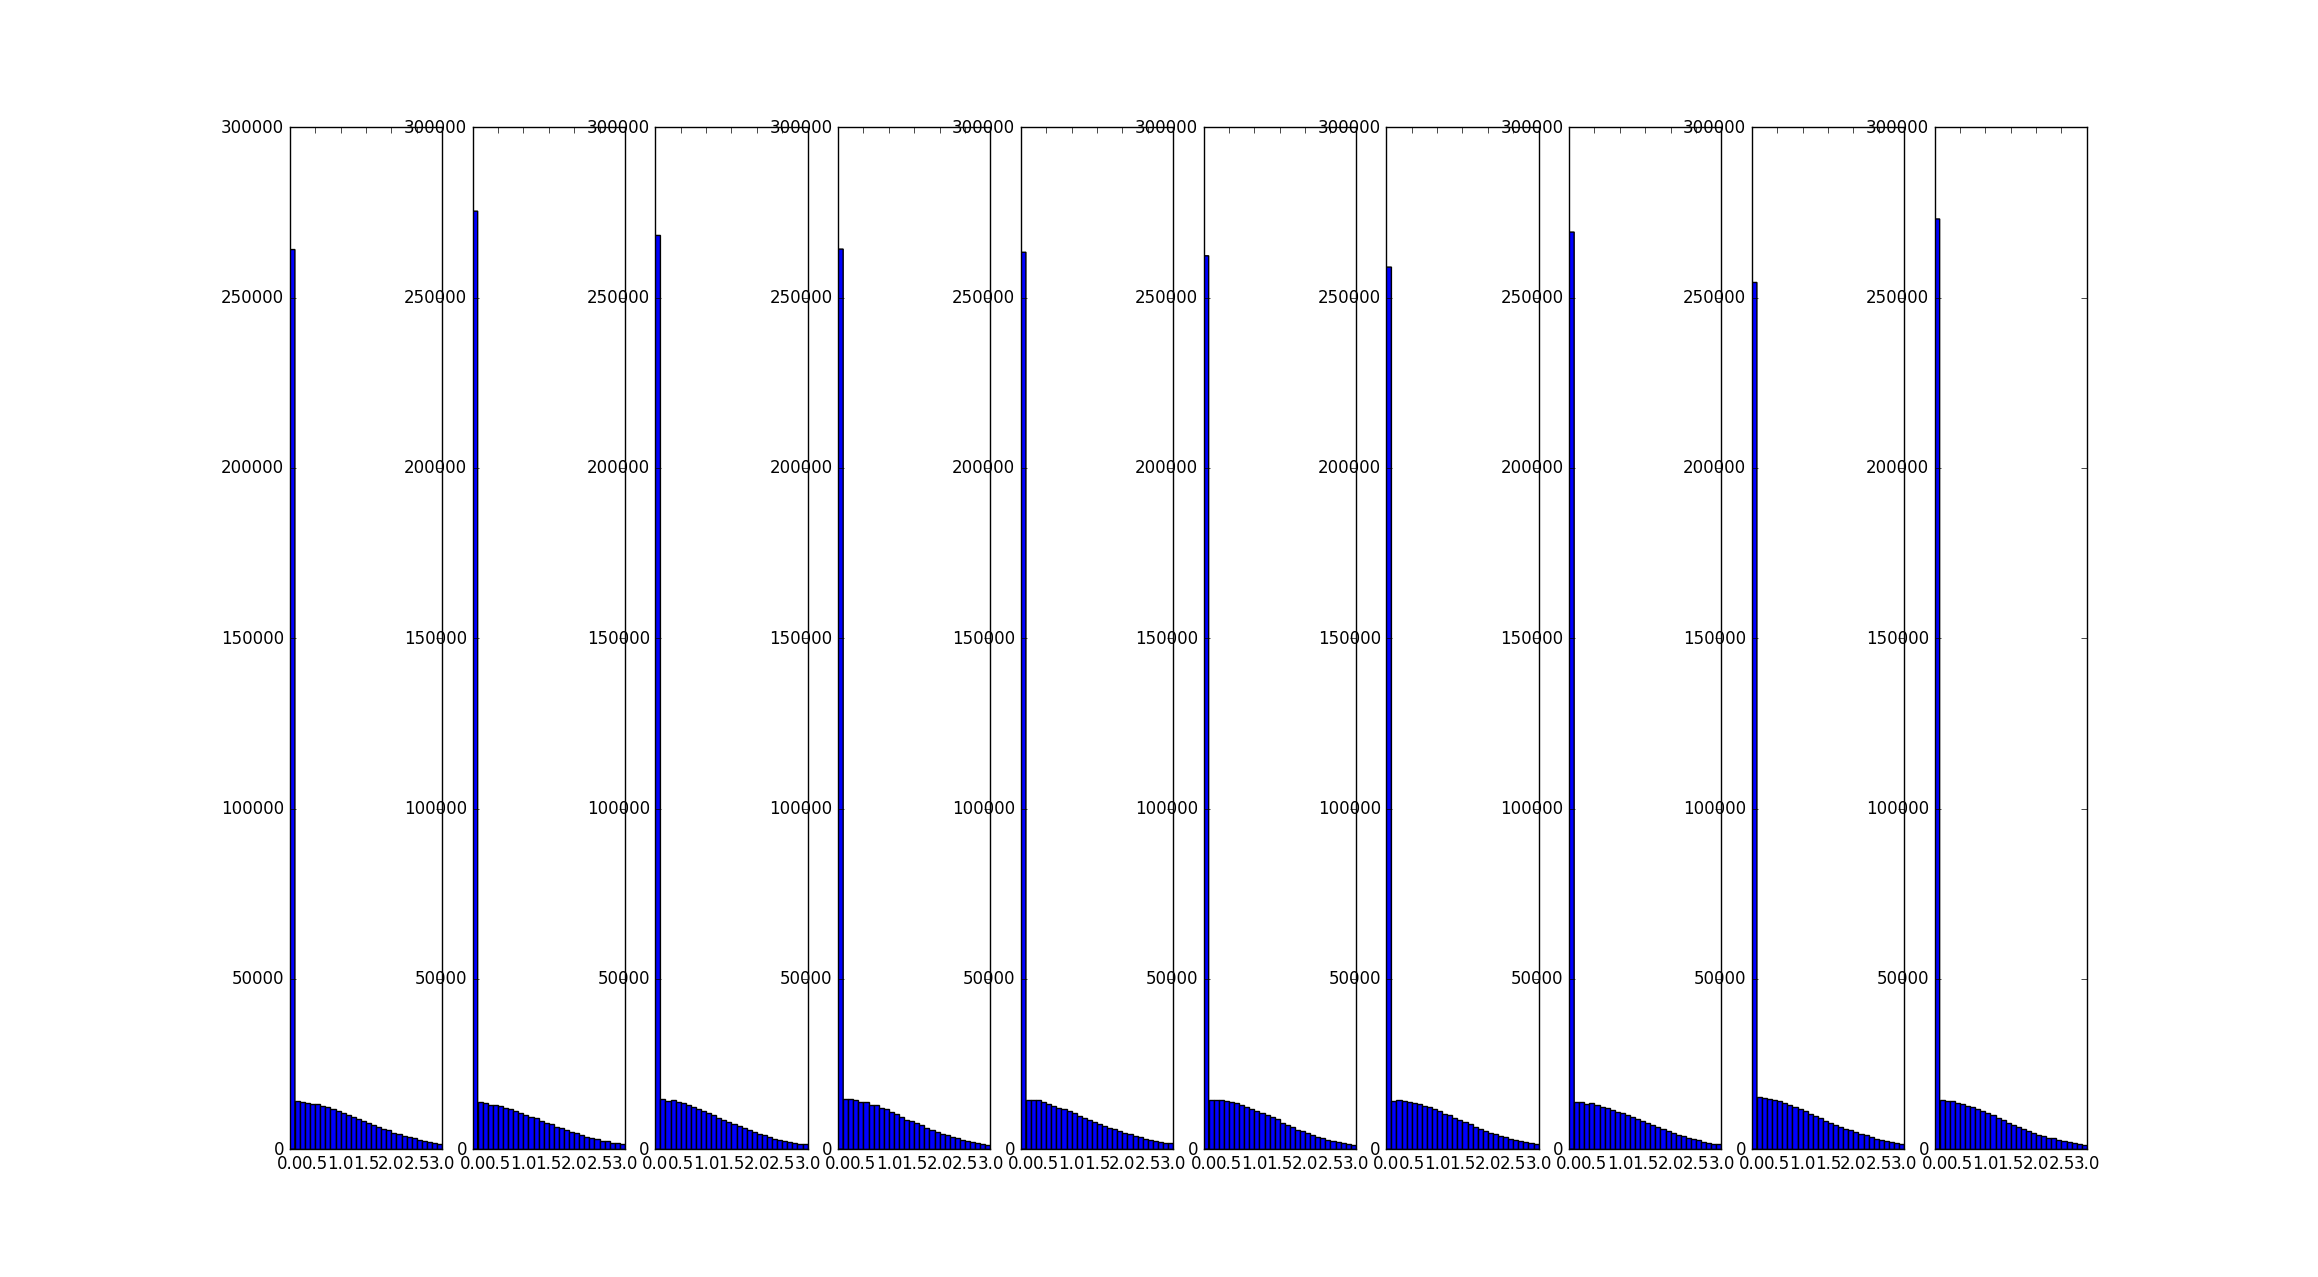
\includegraphics[scale=0.15]{./images/relu_plts_sqrt2.png}
						\end{figure}
					}
				}
			\end{overlayarea}
		\end{column}
		\begin{column}{0.5\textwidth}
			\begin{overlayarea}{\textwidth}{\textheight}
				
				\only<1-2>{
					\begin{itemize}
						\justifying
						\only<1->{\item Indeed when we account for this factor of 2 we see better performance}
					\end{itemize}
				}
			\end{overlayarea}
		\end{column}
	\end{columns}
\end{frame}